\section{Cải thiện chuyển giao tấn công}
Trong tài liệu (Carlini and Wagner 2017b) đã chỉ ra rằng tấn công C\&W có khả năng chuyển giao tốt hơn  từ 1 mạng không phòng thủ sang 1 mạng chắt lọc phòng thủ bằng cách tối ưu tham số độ tin cậy $\kappa$ trong \ref{eq:4}. Theo (Carlini and Wagner 2017b), tác giả sử dụng cùng bộ tham số của chuyển giao tấn công trên tập MNIST, vì MNIST là tập dữ liệu khó tấn công nhất về phương diện nhiễu trung bình trên mỗi điểm ảnh như trong bảng \ref{tab:tab_2} ở trên.

Cố định $\kappa$, các mẫu đối nghịch được sinh ra từ mạng gốc (không phòng thủ) được sử dụng để tấn công mạng chắt lọc phòng thủ với tham số nhiệt $T = 100$ (Papernot et al. 2016b). Tỷ lệ tấn công thành công (ASR) của các phương pháp EAD, C\&W và I-FGM được trình bày trong hình \ref{fig:fg_04}. Khi $\kappa = 0$, tất cả các phương pháp đều cho ASR thấp và do đó không tạo được các mẫu đối nghịch có thể chuyển giao. Tỷ lệ ASR của phương pháp EAD và C\&W tăng lên khi đặt $\kappa > 0$ , trong khi đó tỷ lệ ASR của I-FGM thấp (dưới $2\%$) do tấn công này không có các tham số tương tự để có thể chuyển giao.

Chú ý rằng, EAD có thể thu được ASR gần đạt $99\%$ khi $\kappa = 50$, trong khi đó ASR cao nhất mà phương pháp C\&W đạt được là gần $88\%$ khi $\kappa = 40$. Chứng tỏ rằng, khả năng chuyển giao tấn công tăng lên khi sử dụng các mẫu đối nghịch được tạo từ EAD, điều này là do thuật toán ISTA trong phương trình \ref{eq:8} mạnh hơn so với tấn công C\&W qua phương pháp biến đổi theo ngưỡng. Tác giả cũng thấy rằng khi đặt $\kappa$ quá lớn sẽ làm giảm ASR của các chuyển giao tấn công cả bằng phương pháp EAD và lẫn C\&W, do thuật toán tối ưu không tìm được mẫu đối nghịch có thể làm tối thiểu hàm mất mát $f$ trong \ref{eq:4} khi $\kappa$ lớn. Kết quả đầy đủ về khả năng chuyển giao tấn công được báo cáo trong tài liệu mở rộng.

\begin{figure}[H] % places figure environment here   
    \centering % Centers Graphic
    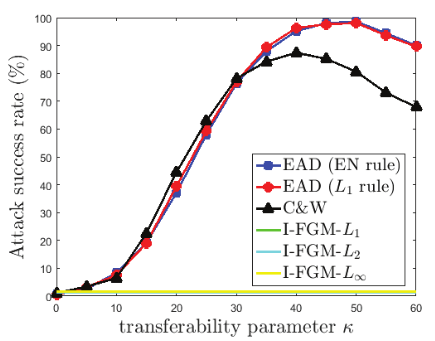
\includegraphics[width=0.5\textwidth]{assets/fig_04.png} 
    \caption{Khả năng chuyển giao tấn công (trường hợp trung bình) từ mạng không phòng thủ sang mạng chắt lọc phòng thủ  trên tập dữ liệu MNIST với các tham số $\kappa$ khác nhau. EAD có thể đạt ASR gần $99\%$ khi $\kappa = 50$, trong khi ASR lớn nhất của C\&W là gần $88\%$ khi $\kappa=40$.} % Creates caption  % Creates caption underneath graph
    \label{fig:fg_04}
\end{figure}